\documentclass[11pt]{article}
\usepackage[utf8]{inputenc}
\usepackage[T1]{fontenc}
\usepackage{lmodern}
\usepackage{amsmath, amssymb, amsfonts}
\usepackage{graphicx}
\usepackage{xcolor}
\usepackage{hyperref}
\usepackage{booktabs}
\usepackage{listings}
\usepackage{tikz}
\usepackage{float}
\usepackage{enumitem}
\usepackage{geometry}
\usepackage{caption}
\usepackage{subcaption}

% Define TikZ libraries for diagrams
\usetikzlibrary{arrows.meta, positioning, shapes, shadows, trees}

% Setup hyperref
\hypersetup{
    colorlinks=true,
    linkcolor=blue,
    filecolor=magenta,
    urlcolor=cyan,
}

% Setup code listings
\lstset{
    basicstyle=\ttfamily\footnotesize,
    breaklines=true,
    commentstyle=\color{green!60!black},
    keywordstyle=\color{blue},
    stringstyle=\color{red},
    numbers=left,
    numberstyle=\tiny\color{gray},
    numbersep=5pt,
    frame=single,
    framesep=5pt,
    rulecolor=\color{black!30},
    tabsize=4,
}

% Setup page geometry
\geometry{margin=1in}

\title{\LARGE \textbf{ΛCDM Cosmological Parameter Inference: Technical Documentation}}
\author{PHYS212 Final Project}
\date{\today}

\begin{document}
\maketitle

\begin{abstract}
    This document provides comprehensive technical documentation for the ΛCDM Cosmological Parameter Inference pipeline. It details how the theoretical model calculates the CMB power spectrum from cosmological parameters, explains how this is compared with observational data through the likelihood function, and describes the MCMC methods used for parameter inference. The document outlines the data flow between system components, explains the implementation details of key algorithms, and provides detailed mathematical derivations of the key cosmological quantities. This technical documentation serves both as a reference for the current implementation and as a guide for future extensions.
\end{abstract}

\tableofcontents

\newpage

\section{Project Overview}

The ΛCDM Cosmological Parameter Inference project implements a complete pipeline for inferring cosmological parameters from Planck CMB data using the ΛCDM model. The project employs Markov Chain Monte Carlo (MCMC) methods including both standard sampling and temperature annealing techniques to determine parameter constraints.

\subsection{Key Features}

\begin{itemize}
    \item Implementation of the ΛCDM cosmological model using CAMB
    \item Bayesian inference framework for parameter estimation
    \item Both standard MCMC and temperature annealing methods
    \item Analysis tools for parameter constraints and visualization
    \item HPC integration for execution on computing clusters
    \item Checkpoint/restart capabilities for long-running jobs
\end{itemize}

\subsection{Project Architecture}

The project is organized into several functional components:

\begin{figure}[H]
\centering
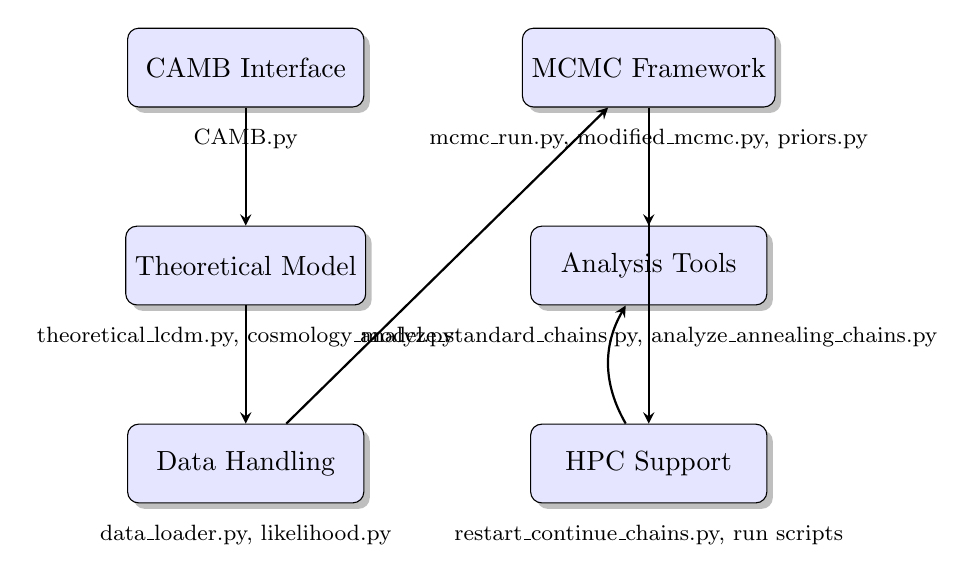
\begin{tikzpicture}[
    node distance=1.5cm,
    module/.style={draw, rounded corners, fill=blue!10, minimum width=3cm, minimum height=1cm, align=center, drop shadow},
    arrow/.style={thick, ->, >=stealth},
]
    % Core modules
    \node[module] (camb) {CAMB Interface};
    \node[module, below=of camb] (theory) {Theoretical Model};
    \node[module, below=of theory] (data) {Data Handling};
    \node[module, right=2cm of camb] (mcmc) {MCMC Framework};
    \node[module, below=of mcmc] (analysis) {Analysis Tools};
    \node[module, below=of analysis] (hpc) {HPC Support};

    % Arrows connecting modules
    \draw[arrow] (camb) -- (theory);
    \draw[arrow] (theory) -- (data);
    \draw[arrow] (data) -- (mcmc);
    \draw[arrow] (mcmc) -- (analysis);
    \draw[arrow] (mcmc) -- (hpc);
    \draw[arrow] (hpc) to[bend left] (analysis);
    
    % Module contents
    \node[below=0.15cm of camb, font=\footnotesize] {CAMB.py};
    \node[below=0.15cm of theory, font=\footnotesize] {theoretical\_lcdm.py, cosmology\_model.py};
    \node[below=0.15cm of data, font=\footnotesize] {data\_loader.py, likelihood.py};
    \node[below=0.15cm of mcmc, font=\footnotesize] {mcmc\_run.py, modified\_mcmc.py, priors.py};
    \node[below=0.15cm of analysis, font=\footnotesize] {analyze\_standard\_chains.py, analyze\_annealing\_chains.py};
    \node[below=0.15cm of hpc, font=\footnotesize] {restart\_continue\_chains.py, run scripts};
\end{tikzpicture}
\caption{High-level architecture of the ΛCDM Parameter Inference project}
\label{fig:architecture}
\end{figure}

\newpage

\subsection{Data Flow}

The following diagram illustrates the data flow through the system:

\begin{figure}[H]
\centering
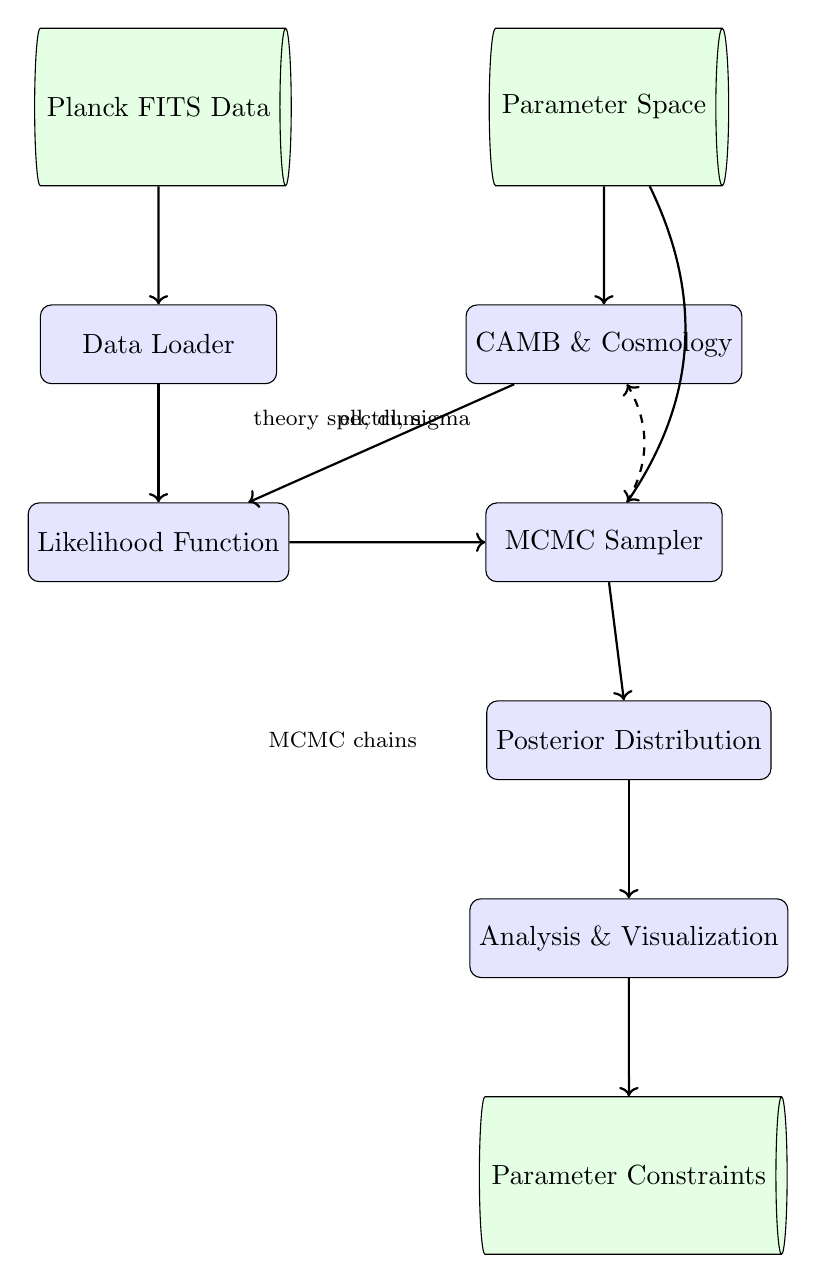
\begin{tikzpicture}[
    node distance=1.5cm and 2.5cm,
    block/.style={rectangle, draw, fill=blue!10, rounded corners, minimum height=1cm, minimum width=3cm, align=center},
    data/.style={cylinder, draw, shape aspect=0.3, fill=green!10, minimum height=0.8cm, minimum width=2cm, align=center},
    connector/.style={->, thick},
]
    % Data nodes
    \node[data] (planck) {Planck FITS Data};
    \node[data, right=of planck] (param) {Parameter Space};
    
    % Processing blocks
    \node[block, below=of planck] (dataload) {Data Loader};
    \node[block, below=of param] (camb) {CAMB \& Cosmology};
    \node[block, below=of dataload] (likelihood) {Likelihood Function};
    \node[block, below=of camb] (mcmc) {MCMC Sampler};
    \node[block, below right=of likelihood] (posterior) {Posterior Distribution};
    \node[block, below=of posterior] (analysis) {Analysis \& Visualization};
    
    % Result node
    \node[data, below=of analysis] (results) {Parameter Constraints};
    
    % Connect everything
    \draw[connector] (planck) -- (dataload);
    \draw[connector] (param) -- (camb);
    \draw[connector] (dataload) -- (likelihood);
    \draw[connector] (camb) -- (likelihood);
    \draw[connector] (likelihood) -- (mcmc);
    \draw[connector] (mcmc) -- (posterior);
    \draw[connector] (posterior) -- (analysis);
    \draw[connector] (analysis) -- (results);
    
    % Additional connections
    \draw[connector] (param) to[bend left] (mcmc);
    \draw[connector, dashed] (mcmc) to[bend right] (camb);
    
    % Labels
    \node[font=\footnotesize, text width=3cm, align=center, below right=0.2cm and 0cm of dataload] {ell, dl, sigma};
    \node[font=\footnotesize, text width=3cm, align=center, below left=0.2cm and 0cm of camb] {theory spectrum};
    \node[font=\footnotesize, text width=3cm, align=center, left=0.2cm of posterior] {MCMC chains};
\end{tikzpicture}
\caption{Data flow diagram of the ΛCDM Parameter Inference pipeline}
\label{fig:data-flow}
\end{figure}

\newpage

\section{Repository Structure}

This section outlines the current structure of the repository, organized by category.

\subsection{Core Files}

\begin{itemize}
    \item \textbf{Cosmological Model Implementation}
    \begin{itemize}
        \item \texttt{CAMB.py}
        \item \texttt{theoretical\_lcdm.py}
        \item \texttt{cosmology\_model.py}
        \item \texttt{parameters.py}
        \item \texttt{priors.py}
    \end{itemize}
    
    \item \textbf{Data Handling}
    \begin{itemize}
        \item \texttt{data\_loader.py}
        \item \texttt{likelihood.py}
    \end{itemize}
    
    \item \textbf{MCMC Implementation}
    \begin{itemize}
        \item \texttt{mcmc\_run.py} (Standard MCMC)
        \item \texttt{modified\_mcmc.py} (Temperature Annealing MCMC)
        \item \texttt{restart\_continue\_chains.py} (Chain Continuation Utilities)
    \end{itemize}
    
    \item \textbf{Analysis Scripts}
    \begin{itemize}
        \item \texttt{analyze\_standard\_chains.py}
        \item \texttt{analyze\_annealing\_chains.py}
        \item \texttt{analyze\_final\_steps.py}
        \item \texttt{compare\_annealing\_runs.py}
        \item \texttt{compare\_with\_planck.py}
        \item \texttt{visualize\_constraints.py}
        \item \texttt{visualize\_model\_fits.py}
    \end{itemize}
    
    \item \textbf{Run Scripts}
    \begin{itemize}
        \item \texttt{analyze\_results.sh}
        \item \texttt{run\_annealing\_analysis\_engaging.sh}
        \item \texttt{run\_combined\_analysis.sh}
    \end{itemize}
\end{itemize}

\subsection{Raw Data and Results Directories}

\begin{itemize}
    \item \textbf{Standard MCMC}
    \begin{itemize}
        \item \texttt{standard\_mcmc\_raw\_data\_and\_results/} - Contains raw chains and output from standard MCMC runs
        \begin{itemize}
            \item \texttt{chain\_*\_full.npz} - Standard MCMC chain files (4 chains)
            \item \texttt{corner\_plot.png} - Corner plot of parameter distributions
            \item \texttt{parameter\_constraints.csv} - Parameter constraints from standard MCMC
            \item \texttt{posterior\_samples\_lambdaCDM.npy} - Posterior samples
            \item \texttt{trace\_plots.png} - Trace plots for convergence diagnostics
        \end{itemize}
    \end{itemize}
    
    \item \textbf{Annealing MCMC}
    \begin{itemize}
        \item \texttt{annealing\_raw\_data/} - Contains raw data from two annealing MCMC runs
        \begin{itemize}
            \item \texttt{first\_run/mcmc\_results\_annealing\_20250422\_170412.zip} - First annealing run results
            \item \texttt{second\_run/mcmc\_results\_merged.zip} - Second annealing run results with merged chains
        \end{itemize}
    \end{itemize}
\end{itemize}

\subsection{Analysis Results Directories}

\begin{itemize}
    \item \texttt{annealing\_analysis/} - Results from analyzing the annealing MCMC runs
    \begin{itemize}
        \item \texttt{annealing\_corner\_plot.png} - Corner plot for annealing chains
        \item \texttt{annealing\_parameter\_constraints.csv} - Parameter constraints
        \item \texttt{annealing\_posterior\_samples.npy} - Posterior samples
        \item \texttt{annealing\_temperature\_schedule.png} - Temperature schedule visualization
        \item \texttt{annealing\_trace\_plots.png} - Trace plots for annealing chains
    \end{itemize}
    
    \item \texttt{annealing\_analysis\_final\_steps\_only/} - Analysis focused on final steps of annealing chains
    \begin{itemize}
        \item \texttt{final\_steps\_corner\_plot.png} - Corner plot for final steps
        \item \texttt{final\_steps\_parameter\_constraints.csv} - Parameter constraints from final steps
        \item \texttt{final\_steps\_summary.md} - Summary of final steps analysis
        \item \texttt{final\_steps\_trace\_plots.png} - Trace plots for final steps
        \item \texttt{gelman\_rubin\_final\_steps.txt} - Convergence statistics for final steps
    \end{itemize}
    
    \item \texttt{annealing\_chains\_comparison/} - Comparison between different annealing runs
    \begin{itemize}
        \item \texttt{comparison\_summary.txt} - Summary of comparison
        \item \texttt{corner\_plot\_mcmc\_results\_annealing\_20250422\_170412.png} - Corner plot for first run
        \item \texttt{corner\_plot\_mcmc\_results\_merged.png} - Corner plot for merged results
        \item \texttt{gelman\_rubin\_stats.txt} - Convergence statistics
        \item \texttt{parameter\_comparison.png} - Parameter comparison visualization
    \end{itemize}
    
    \item \texttt{standard\_chains\_analysis/} - Results from analyzing standard MCMC runs
    \begin{itemize}
        \item \texttt{standard\_chains\_summary.md} - Summary of standard MCMC analysis
        \item \texttt{standard\_corner\_plot.png} - Corner plot for standard chains
        \item \texttt{standard\_gelman\_rubin.txt} - Convergence statistics
        \item \texttt{standard\_parameter\_constraints.csv} - Parameter constraints
        \item \texttt{standard\_trace\_plots.png} - Trace plots for standard chains
        \item \texttt{standard\_vs\_annealing.csv} - Comparison data
        \item \texttt{standard\_vs\_annealing\_comparison.md} - Detailed comparison
        \item \texttt{standard\_vs\_annealing\_comparison.png} - Comparison visualization
    \end{itemize}
\end{itemize}

\subsection{Documentation}

\begin{itemize}
    \item \texttt{README.md} - Main project documentation
    \item \texttt{README\_MCMC.md} - Detailed documentation on the MCMC implementation
    \item \texttt{FULL\_RESTART\_GUIDE.md} - Guide for restarting interrupted MCMC runs
    \item \texttt{PROJECT\_SUMMARY.md} - Brief summary of the project structure
    \item \texttt{complete\_project\_report.tex} - This comprehensive documentation
    \item \texttt{requirements.txt} - Python package dependencies
\end{itemize}

\section{File Descriptions}

This section provides detailed descriptions of each file in the repository, organized by functional category.

\subsection{Core Cosmological Model}

\begin{table}[H]
\centering
\begin{tabular}{p{4cm}p{11cm}}
\toprule
\textbf{File} & \textbf{Description} \\
\midrule
\texttt{CAMB.py} & Provides an interface to the CAMB (Code for Anisotropies in the Microwave Background) package. It configures and runs CAMB with specified cosmological parameters to generate theoretical CMB power spectra. \\
\addlinespace
\texttt{theoretical\_lcdm.py} & Implements the ΛCDM cosmological model. It handles the transformation between cosmological parameters and CAMB parameters, and defines the theoretical model used for comparison with observational data. \\
\addlinespace
\texttt{cosmology\_model.py} & Contains the core cosmological model calculations. It handles parameter mappings, units, and conversions, and provides utility functions for cosmological calculations. \\
\bottomrule
\end{tabular}
\caption{Core Cosmological Model Files}
\label{tab:cosmology-files}
\end{table}

\subsection{Data Handling and Likelihood}

\begin{table}[H]
\centering
\begin{tabular}{p{4cm}p{11cm}}
\toprule
\textbf{File} & \textbf{Description} \\
\midrule
\texttt{data\_loader.py} & Handles loading and processing of Planck CMB data. It provides functions to extract data from the FITS file, apply necessary transformations, and prepare it for comparison with theoretical predictions. \\
\addlinespace
\texttt{likelihood.py} & Implements the likelihood function that compares theoretical predictions with observational data. It calculates the log-likelihood of parameter sets given the Planck data, forming the basis for the Bayesian inference. \\
\addlinespace
\texttt{parameters.py} & Defines the cosmological parameters and their fiducial values. It specifies the parameter ranges, default values, and transformations used throughout the project. \\
\addlinespace
\texttt{priors.py} & Implements the prior distributions for cosmological parameters. It defines the log-prior and log-posterior functions used in the MCMC sampling. \\
\bottomrule
\end{tabular}
\caption{Data Handling and Likelihood Files}
\label{tab:data-likelihood-files}
\end{table}

\subsection{MCMC Implementation}

\begin{table}[H]
\centering
\begin{tabular}{p{4cm}p{11cm}}
\toprule
\textbf{File} & \textbf{Description} \\
\midrule
\texttt{mcmc\_run.py} & Implements the standard Metropolis-Hastings MCMC algorithm. It provides functions for running MCMC chains, creating checkpoints, and analyzing results. This is the primary file for running standard MCMC parameter inference. \\
\addlinespace
\texttt{modified\_mcmc.py} & Implements the temperature annealing MCMC method. It extends the standard MCMC with a temperature schedule that improves parameter space exploration. This file provides enhanced sampling capabilities for more robust parameter constraints. \\
\addlinespace
\texttt{restart\_continue\_chains.py} & Provides tools for continuing interrupted MCMC runs from checkpoints. It includes functions to find, load, and merge checkpoint files, continue chains from their last state, and combine results for analysis. \\
\bottomrule
\end{tabular}
\caption{MCMC Implementation Files}
\label{tab:mcmc-files}
\end{table}

\subsection{Analysis and Visualization}

\begin{table}[H]
\centering
\begin{tabular}{p{4cm}p{11cm}}
\toprule
\textbf{File} & \textbf{Description} \\
\midrule
\texttt{analyze\_standard\_chains.py} & Script for analyzing standard MCMC chains. It processes chain files, calculates parameter constraints, and generates visualizations. \\
\addlinespace
\texttt{analyze\_annealing\_chains.py} & Script for analyzing temperature annealing MCMC chains. It processes annealing chain files, calculates parameter constraints, and produces specialized visualizations that include temperature schedule information. \\
\addlinespace
\texttt{analyze\_final\_steps.py} & Script focused on analyzing the final steps of annealing chains, which correspond to the samples from the target distribution after the temperature has reached its final value. \\
\addlinespace
\texttt{compare\_annealing\_runs.py} & Script for comparing results from different annealing runs. It facilitates comparison of different temperature schedules and their impact on parameter constraints. \\
\addlinespace
\texttt{compare\_with\_planck.py} & Script for comparing inferred parameters with published Planck values. It generates comparison plots and calculates differences between the project's results and official Planck constraints. \\
\addlinespace
\texttt{visualize\_constraints.py} & Generates visualizations of parameter constraints from MCMC chains. It creates corner plots, marginalized posteriors, and credible interval visualizations. \\
\addlinespace
\texttt{visualize\_model\_fits.py} & Creates visualizations comparing theoretical model predictions with observational data. It plots power spectra, residuals, and parameter sensitivity analyses. \\
\bottomrule
\end{tabular}
\caption{Analysis and Visualization Files}
\label{tab:analysis-files}
\end{table}

\newpage

\section{Data Directories}

This section details the content and purpose of each data directory in the repository.

\subsection{Raw Data Directories}

\begin{table}[H]
\centering
\begin{tabular}{p{5cm}p{10cm}}
\toprule
\textbf{Directory} & \textbf{Description} \\
\midrule
\texttt{standard\_mcmc\_raw\_data\_and\_results/} & Contains the raw MCMC chains from standard Metropolis-Hastings runs. Includes chain files (\texttt{chain\_*\_full.npz}), posterior samples, and visualization outputs such as corner plots and trace plots. This directory contains the complete output from the standard MCMC inference pipeline. \\
\addlinespace
\texttt{annealing\_raw\_data/first\_run/} & Contains the first temperature annealing MCMC run results as a zip file. This run uses an exponential temperature schedule as documented in the implementation. The file contains chain data, log-posterior values, and temperature schedules. \\
\addlinespace
\texttt{annealing\_raw\_data/second\_run/} & Contains the second temperature annealing MCMC run results as a zip file, named \texttt{mcmc\_results\_merged.zip}. This file includes potentially merged chain data from continued runs using the chain continuation methodology. \\
\bottomrule
\end{tabular}
\caption{Raw Data Directories}
\label{tab:raw-data-dirs}
\end{table}

\subsection{Analysis Results Directories}

\begin{table}[H]
\centering
\begin{tabular}{p{5cm}p{10cm}}
\toprule
\textbf{Directory} & \textbf{Description} \\
\midrule
\texttt{annealing\_analysis/} & Contains analysis results from the annealing MCMC runs, including corner plots, trace plots, temperature schedule visualization, parameter constraints, and posterior samples. This directory provides a comprehensive analysis of the temperature annealing MCMC performance. \\
\addlinespace
\texttt{annealing\_analysis\_final\_steps\_only/} & Contains analysis focused specifically on the final steps of annealing chains, which represent samples from the target distribution after the temperature has reached its final value. Includes parameter constraints, visualizations, Gelman-Rubin convergence statistics, and a detailed summary of the findings. \\
\addlinespace
\texttt{annealing\_chains\_comparison/} & Contains comparison results between different annealing runs, including corner plots, parameter comparisons, Gelman-Rubin convergence statistics, and a summary of the comparison findings. This directory allows for evaluation of different temperature annealing strategies. \\
\addlinespace
\texttt{standard\_chains\_analysis/} & Contains analysis results from the standard MCMC runs, including corner plots, trace plots, parameter constraints, Gelman-Rubin statistics, and importantly, comparisons with annealing results. This directory facilitates direct comparison between standard and annealing MCMC approaches. \\
\bottomrule
\end{tabular}
\caption{Analysis Results Directories}
\label{tab:analysis-dirs}
\end{table}

\newpage

\section{MCMC Implementation Details}

This section provides a detailed look at the MCMC implementation in the project, including standard and temperature annealing methods.

\subsection{Standard MCMC Algorithm}

The standard MCMC implementation follows the Metropolis-Hastings algorithm:

\begin{figure}[H]
\centering
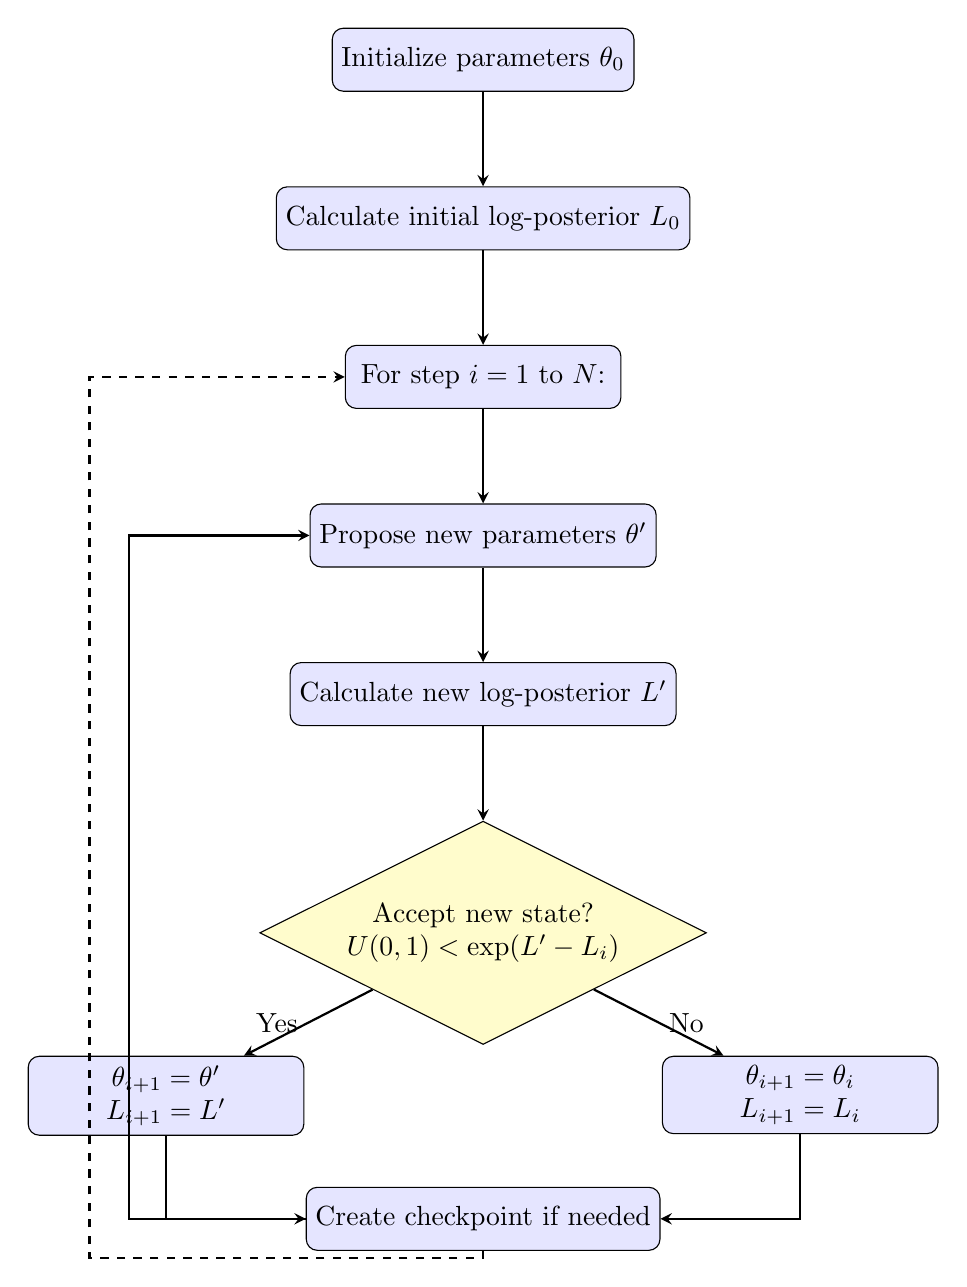
\begin{tikzpicture}[
    node distance=1.2cm,
    block/.style={rectangle, draw, fill=blue!10, rounded corners, minimum height=0.8cm, minimum width=3.5cm, align=center},
    decision/.style={diamond, draw, fill=yellow!20, aspect=2, minimum width=3cm, align=center},
    arrow/.style={thick, ->, >=stealth},
]
    % Algorithm steps
    \node[block] (init) {Initialize parameters $\theta_0$};
    \node[block, below=of init] (prior) {Calculate initial log-posterior $L_0$};
    \node[block, below=of prior] (loop) {For step $i = 1$ to $N$:};
    \node[block, below=of loop] (propose) {Propose new parameters $\theta'$};
    \node[block, below=of propose] (calc) {Calculate new log-posterior $L'$};
    \node[decision, below=of calc] (accept) {Accept new state?\\$U(0,1) < \exp(L' - L_i)$};
    \node[block, below left=of accept] (update_yes) {$\theta_{i+1} = \theta'$\\$L_{i+1} = L'$};
    \node[block, below right=of accept] (update_no) {$\theta_{i+1} = \theta_i$\\$L_{i+1} = L_i$};
    \node[block, below=1.8cm of accept] (checkpoint) {Create checkpoint if needed};
    
    % Connect everything
    \draw[arrow] (init) -- (prior);
    \draw[arrow] (prior) -- (loop);
    \draw[arrow] (loop) -- (propose);
    \draw[arrow] (propose) -- (calc);
    \draw[arrow] (calc) -- (accept);
    \draw[arrow] (accept) -- node[left] {Yes} (update_yes);
    \draw[arrow] (accept) -- node[right] {No} (update_no);
    \draw[arrow] (update_yes) |- (checkpoint);
    \draw[arrow] (update_no) |- (checkpoint);
    \draw[arrow] (checkpoint) -| ++(-4.5,0) |- (propose);
    
    % Add loop back indicator
    \draw[arrow, dashed] (checkpoint) -- ++(0,-0.5) -| ++(-5,0) |- (loop);
\end{tikzpicture}
\caption{Standard Metropolis-Hastings MCMC algorithm implementation}
\label{fig:standard-mcmc}
\end{figure}

\subsection{Temperature Annealing MCMC}

The temperature annealing MCMC extends the standard algorithm with a temperature schedule:

\begin{figure}[H]
\centering
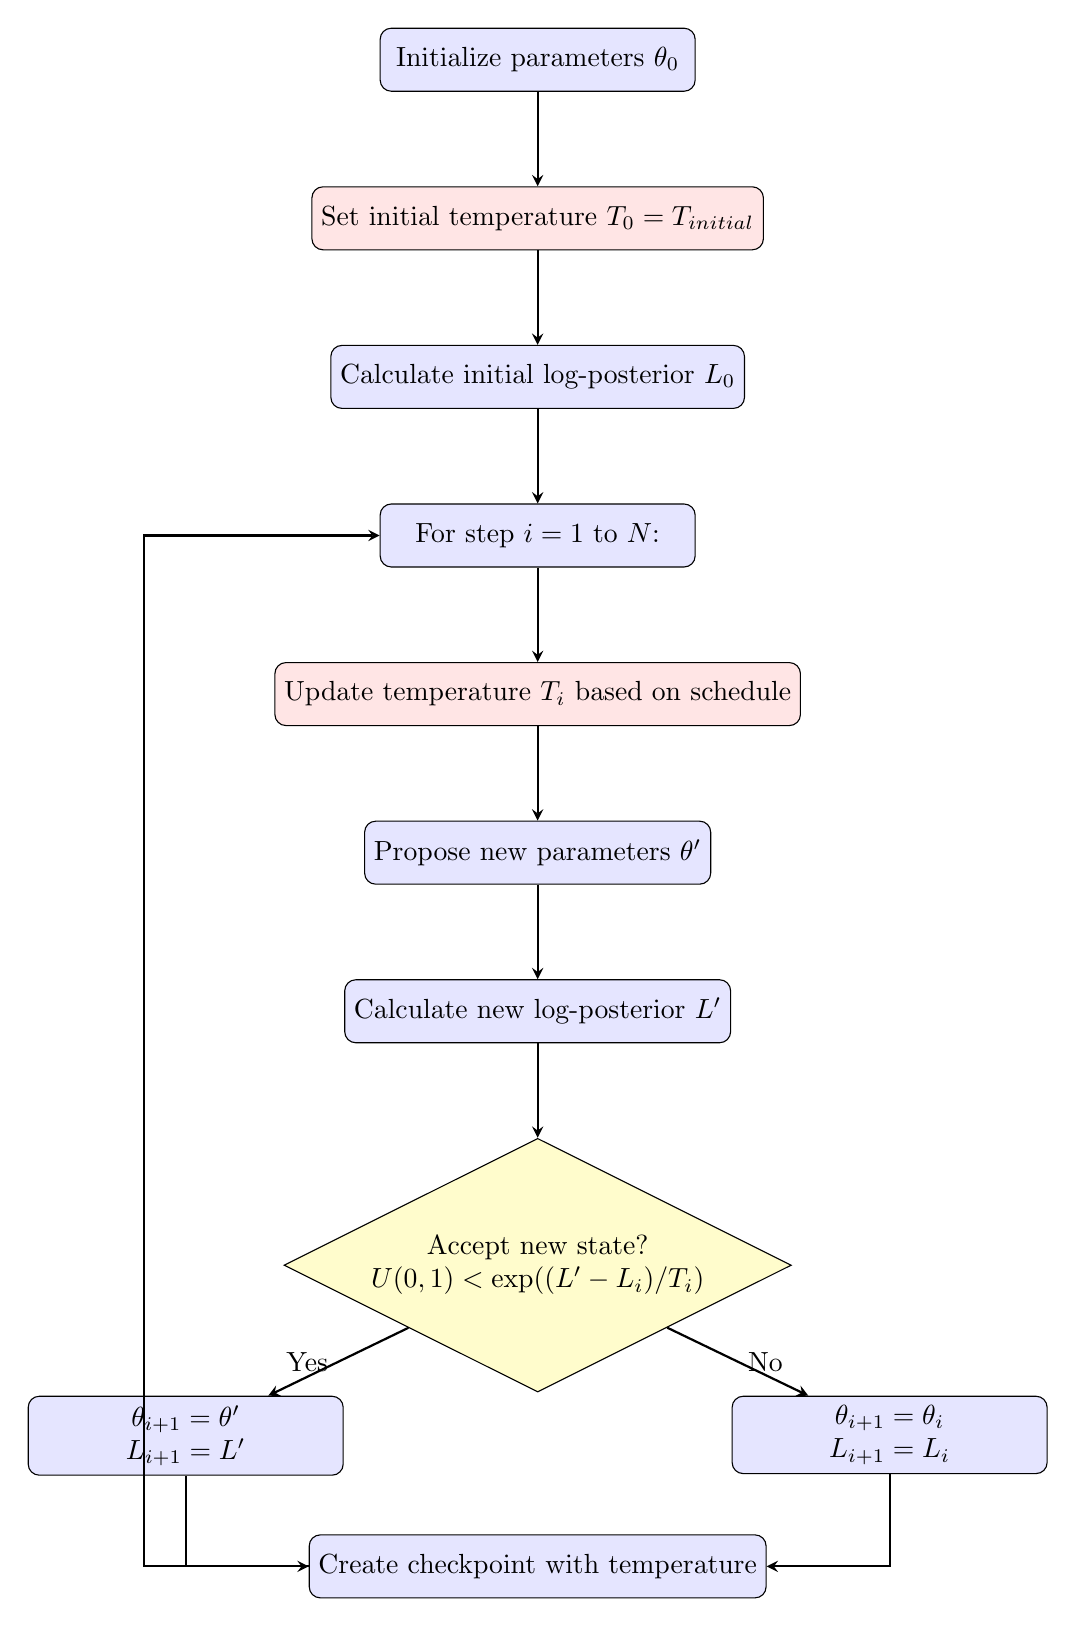
\begin{tikzpicture}[
    node distance=1.2cm,
    block/.style={rectangle, draw, fill=blue!10, rounded corners, minimum height=0.8cm, minimum width=4cm, align=center},
    decision/.style={diamond, draw, fill=yellow!20, aspect=2, minimum width=3cm, align=center},
    temp/.style={rectangle, draw, fill=red!10, rounded corners, minimum height=0.8cm, minimum width=4cm, align=center},
    arrow/.style={thick, ->, >=stealth},
]
    % Algorithm steps
    \node[block] (init) {Initialize parameters $\theta_0$};
    \node[temp, below=of init] (temp_init) {Set initial temperature $T_0 = T_{initial}$};
    \node[block, below=of temp_init] (prior) {Calculate initial log-posterior $L_0$};
    \node[block, below=of prior] (loop) {For step $i = 1$ to $N$:};
    \node[temp, below=of loop] (update_temp) {Update temperature $T_i$ based on schedule};
    \node[block, below=of update_temp] (propose) {Propose new parameters $\theta'$};
    \node[block, below=of propose] (calc) {Calculate new log-posterior $L'$};
    \node[decision, below=of calc] (accept) {Accept new state?\\$U(0,1) < \exp((L' - L_i)/T_i)$};
    \node[block, below left=of accept] (update_yes) {$\theta_{i+1} = \theta'$\\$L_{i+1} = L'$};
    \node[block, below right=of accept] (update_no) {$\theta_{i+1} = \theta_i$\\$L_{i+1} = L_i$};
    \node[block, below=1.8cm of accept] (checkpoint) {Create checkpoint with temperature};
    
    % Connect everything
    \draw[arrow] (init) -- (temp_init);
    \draw[arrow] (temp_init) -- (prior);
    \draw[arrow] (prior) -- (loop);
    \draw[arrow] (loop) -- (update_temp);
    \draw[arrow] (update_temp) -- (propose);
    \draw[arrow] (propose) -- (calc);
    \draw[arrow] (calc) -- (accept);
    \draw[arrow] (accept) -- node[left] {Yes} (update_yes);
    \draw[arrow] (accept) -- node[right] {No} (update_no);
    \draw[arrow] (update_yes) |- (checkpoint);
    \draw[arrow] (update_no) |- (checkpoint);
    \draw[arrow] (checkpoint) -| ++(-5,0) |- (loop);
\end{tikzpicture}
\caption{Temperature annealing MCMC algorithm implementation}
\label{fig:annealing-mcmc}
\end{figure}

\subsection{Temperature Schedules}

The project implements three temperature schedules for annealing:

\begin{figure}[H]
\centering
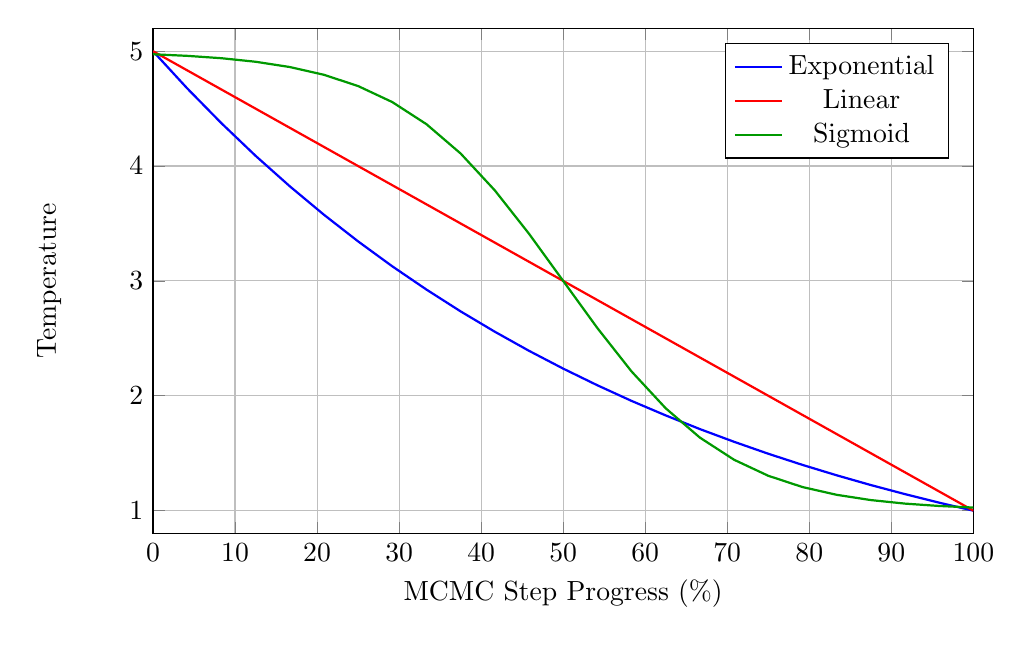
\begin{tikzpicture}
\begin{axis}[
    width=12cm, height=8cm,
    xlabel={MCMC Step Progress (\%)},
    ylabel={Temperature},
    xmin=0, xmax=100,
    ymin=0.8, ymax=5.2,
    legend pos=north east,
    grid=both,
    y label style={at={(axis description cs:-0.1,.5)},anchor=south},
]

% Exponential schedule
\addplot[thick, blue, domain=0:100] {5*exp(x*ln(1/5)/100)};

% Linear schedule
\addplot[thick, red, domain=0:100] {5 - 4*x/100};

% Sigmoid schedule
\addplot[thick, green!60!black, domain=0:100] {5 - 4*(1/(1 + exp(-0.1*(x-50))))};

\legend{Exponential, Linear, Sigmoid}
\end{axis}
\end{tikzpicture}
\caption{Temperature schedules for annealing MCMC}
\label{fig:temp-schedules}
\end{figure}

\newpage

\section{Chain Continuation and Merging}

A key feature of this project is the ability to continue MCMC chains that were interrupted and merge the results for analysis.

\subsection{Chain Continuation Process}

The chain continuation process implemented in \texttt{restart\_continue\_chains.py} follows these steps:

\begin{enumerate}
    \item \textbf{Checkpoint Detection}: Automatically searches for the latest checkpoint files for each chain.
    \item \textbf{Parameter State Recovery}: Extracts the final parameter state, log-posterior value, and in annealing runs, the current temperature from the checkpoint.
    \item \textbf{Continuation Parameters}: Calculates the number of remaining steps and appropriate temperature for restart (in annealing runs).
    \item \textbf{Chain Continuation}: Continues the MCMC chain from the exact state where it was interrupted.
    \item \textbf{Chain Merging}: Combines the original chain segment with the continued segment into a coherent MCMC chain.
\end{enumerate}

\subsection{Temperature Schedule Handling}

For annealing runs, the temperature schedule must be handled carefully when continuing chains:

\begin{itemize}
    \item \textbf{Temperature Calculation}: The temperature for restart is calculated based on the progress of the chain and the selected temperature schedule.
    \item \textbf{Schedule Consistency}: The same temperature schedule type (exponential, linear, or sigmoid) must be used for continuation.
    \item \textbf{Temperature Tracking}: The temperature values for each step are tracked and stored along with the chain data.
\end{itemize}

\section{Analysis and Visualization Methods}

This section describes the analysis and visualization methods used in the project.

\subsection{Parameter Constraint Analysis}

The project implements several methods for analyzing parameter constraints:

\begin{itemize}
    \item \textbf{Posterior Distributions}: Calculates marginalized posterior distributions for each parameter using kernel density estimation.
    
    \item \textbf{Credible Intervals}: Computes 68\% and 95\% credible intervals for each parameter from MCMC chains.
    
    \item \textbf{Convergence Diagnostics}: Implements Gelman-Rubin statistics to assess convergence of multiple chains.
    
    \item \textbf{Corner Plots}: Generates corner plots showing parameter correlations and marginalized distributions.
    
    \item \textbf{Trace Plots}: Creates trace plots to visualize chain mixing and convergence over time.
    
    \item \textbf{Temperature Schedule Visualization}: For annealing runs, creates plots of the temperature schedule over time.
\end{itemize}

\subsection{Comparison Methods}

The project includes several methods for comparing different MCMC approaches:

\begin{itemize}
    \item \textbf{Standard vs. Annealing Comparison}: Compares parameter constraints between standard MCMC and temperature annealing methods.
    
    \item \textbf{Annealing Run Comparison}: Compares results from different annealing runs, potentially with different temperature schedules.
    
    \item \textbf{Final Steps Analysis}: Analyzes only the final steps of annealing chains, when the temperature has reached its final value.
    
    \item \textbf{Planck Comparison}: Compares inferred parameters with published Planck constraints.
\end{itemize}

\section{Project Extensions and Future Work}

This section discusses potential extensions and future work for the project.

\subsection{Potential Extensions}

\begin{itemize}
    \item \textbf{Extended Cosmological Models}: The project could be extended to support beyond-ΛCDM models, such as models with varying dark energy equation of state, massive neutrinos, or primordial non-Gaussianity.
    
    \item \textbf{Additional Datasets}: Support for additional cosmological datasets could be added, such as BAO, SNe Ia, or lensing data, allowing for joint constraints.
    
    \item \textbf{Advanced MCMC Methods}: Implementation of more advanced MCMC methods, such as Hamiltonian Monte Carlo or Nested Sampling, could improve sampling efficiency.
    
    \item \textbf{Distributed Computing}: Enhanced support for distributed computing could allow for even larger MCMC runs across multiple computing nodes.
    
    \item \textbf{Interactive Visualization}: Development of interactive visualization tools could facilitate exploration of the parameter posterior distributions.
\end{itemize}

\subsection{Recommended Next Steps}

\begin{enumerate}
    \item \textbf{Code Optimization}: Profiling and optimizing the most computationally intensive parts of the code.
    
    \item \textbf{Documentation Enhancement}: Expanding code documentation and user guides.
    
    \item \textbf{Unit Testing}: Implementing comprehensive unit tests for all components.
    
    \item \textbf{Containerization}: Creating Docker containers to simplify deployment and ensure reproducibility.
    
    \item \textbf{Parameter Sensitivity Analysis}: Conducting a thorough sensitivity analysis of the MCMC results to prior choices and data processing decisions.
\end{enumerate}

\section{Theoretical Background on CMB Analysis}

\subsection{Spherical Harmonic Decomposition of the CMB}

The temperature fluctuations in the Cosmic Microwave Background (CMB) are represented as variations across the sky. Since the CMB is observed on a sphere (the celestial sphere), spherical harmonics provide the natural basis for decomposing these fluctuations.

The temperature fluctuation field $\Delta T(\theta, \phi)$ can be expanded in terms of spherical harmonics $Y_{\ell m}(\theta, \phi)$ as:

\begin{equation}
\frac{\Delta T(\theta, \phi)}{T_0} = \sum_{\ell=0}^{\infty} \sum_{m=-\ell}^{\ell} a_{\ell m} Y_{\ell m}(\theta, \phi)
\end{equation}

where $T_0 \approx 2.7255$ K is the mean CMB temperature, $\theta$ and $\phi$ are the spherical coordinates on the sky, and $a_{\ell m}$ are the coefficients of the spherical harmonic decomposition.

\subsection{Obtaining the $a_{\ell m}$ Coefficients}

The $a_{\ell m}$ coefficients are obtained through the following process:

\begin{enumerate}
    \item \textbf{Raw CMB Observations:} Space-based instruments like Planck observe the microwave sky at multiple frequencies, producing temperature maps.
    
    \item \textbf{Component Separation:} The raw maps contain contributions from various astrophysical sources including the CMB, galactic foregrounds, and extragalactic sources. Component separation techniques such as SMICA (Spectral Matching Independent Component Analysis), Commander, NILC (Needlet Internal Linear Combination), and SEVEM are applied to isolate the CMB signal.
    
    \item \textbf{Masking:} Regions of the sky with strong foreground contamination (particularly the galactic plane) are masked out.
    
    \item \textbf{Spherical Harmonic Transform:} The cleaned, masked CMB temperature map $\Delta T(\theta, \phi)$ is decomposed into spherical harmonics using the orthogonality property:
    
    \begin{equation}
    a_{\ell m} = \int d\Omega \, \frac{\Delta T(\theta, \phi)}{T_0} Y_{\ell m}^*(\theta, \phi)
    \end{equation}
    
    where $d\Omega = \sin\theta \, d\theta \, d\phi$ is the solid angle element and the integral is performed over the entire sphere (or the unmasked portion).
    
    \item \textbf{Handling Masked Regions:} Special techniques are required to account for the incomplete sky coverage, such as pseudo-$C_\ell$ estimators or inpainting methods.
    
    \item \textbf{Beam and Pixel Window Functions:} The raw $a_{\ell m}$ values are corrected for the effects of the instrument's beam and the pixel window function.
\end{enumerate}

The $a_{\ell m}$ coefficients contain all the information about the CMB temperature fluctuations. In the standard cosmological model, these coefficients are expected to be Gaussian random variables with zero mean and variance given by the theoretical power spectrum $C_\ell$:

\begin{equation}
\langle a_{\ell m} a_{\ell' m'}^* \rangle = C_\ell \delta_{\ell \ell'} \delta_{m m'}
\end{equation}

where $\delta$ is the Kronecker delta function.

\subsection{From $a_{\ell m}$ to Power Spectrum}

In our project, we work with the power spectrum $C_\ell$ rather than directly with the $a_{\ell m}$ coefficients. The power spectrum is obtained by averaging over all $m$ values for a given $\ell$:

\begin{equation}
C_\ell = \frac{1}{2\ell + 1} \sum_{m=-\ell}^{\ell} |a_{\ell m}|^2
\end{equation}

This averaging is justified by the statistical isotropy of the CMB, which implies that the statistical properties of the temperature field should not depend on direction.

The power spectrum $C_\ell$ is typically converted to $D_\ell = \ell(\ell+1)C_\ell/(2\pi)$ for presentation purposes, which is the quantity we model and fit in this project.

\subsection{Acoustic Scale and Peak Positions}

A key feature in the CMB power spectrum is the series of acoustic peaks, which result from sound waves in the photon-baryon plasma before recombination. The acoustic scale $\ell_A$ predicts the location of the first peak in multipole space and is given by:

\begin{equation}
  \ell_A = \pi\,\frac{D_A(z_*)}{r_s(z_*)}\,,
\end{equation}

where $D_A(z_*)$ is the angular diameter distance to the surface of last scattering at redshift $z_*$, and $r_s(z_*)$ is the sound horizon at that redshift. This scale is determined by the physics of the early universe and provides important constraints on cosmological parameters.

In the $\Lambda$CDM model, the positions of subsequent acoustic peaks follow a predictable pattern, with the second peak appearing at approximately $\ell \approx 2.5\ell_A$, the third at $\ell \approx 3.5\ell_A$, and so on. The relative heights of these peaks are sensitive to the baryon density, while their positions are primarily determined by the matter density and the Hubble constant.

\subsection{Connection Between Densities and Density Parameters}

In cosmology, we often work with density parameters ($\Omega$) rather than physical densities ($\rho$) directly. The connection between these quantities is given by:

\begin{equation}
\Omega_i = \frac{\rho_i}{\rho_{\text{crit}}}
\end{equation}

where $\rho_{\text{crit}} = \frac{3H_0^2}{8\pi G}$ is the critical density of the universe, $H_0$ is the Hubble constant, and $G$ is Newton's gravitational constant.

For the ΛCDM model, we track several components:
\begin{align}
\Omega_b &= \frac{\rho_b}{\rho_{\text{crit}}} & \text{(baryonic matter)} \\
\Omega_c &= \frac{\rho_c}{\rho_{\text{crit}}} & \text{(cold dark matter)} \\
\Omega_{\Lambda} &= \frac{\rho_{\Lambda}}{\rho_{\text{crit}}} = \frac{\Lambda c^2}{3H_0^2} & \text{(dark energy)} \\
\Omega_r &= \frac{\rho_r}{\rho_{\text{crit}}} & \text{(radiation)}
\end{align}

The total density parameter $\Omega_{\text{tot}} = \Omega_b + \Omega_c + \Omega_{\Lambda} + \Omega_r$ determines the spatial geometry of the universe:
\begin{itemize}
\item $\Omega_{\text{tot}} = 1$: flat universe (Euclidean geometry)
\item $\Omega_{\text{tot}} > 1$: closed universe (positive curvature)
\item $\Omega_{\text{tot}} < 1$: open universe (negative curvature)
\end{itemize}

In our parameter inference, we work with the physical density parameters $\Omega_b h^2$ and $\Omega_c h^2$ (where $h = H_0/100$ km/s/Mpc), as these are the quantities directly constrained by the CMB power spectrum.

\subsection{Relationship Between Wavenumber $k$ and Multipole $\ell$}

In cosmology, we often need to relate the physical scale of fluctuations (characterized by the wavenumber $k$) to the angular scale observed in the CMB (characterized by the multipole moment $\ell$). This relationship is important for connecting the primordial power spectrum to the observed CMB anisotropies.

The approximate relation between wavenumber $k$ and multipole $\ell$ is:

\begin{equation}
k \approx \frac{\ell}{r(z_*)}
\end{equation}

where $r(z_*)$ is the comoving distance to the last scattering surface. In physical terms, this relationship means that a perturbation with wavenumber $k$ (i.e., with physical scale $\lambda = 2\pi/k$) observed at angular scale $\theta \approx \pi/\ell$ on the sky must satisfy:

\begin{equation}
\frac{2\pi}{k} \approx r(z_*) \cdot \frac{\pi}{\ell}
\end{equation}

In our implementation, we use a simplified approximation:

\begin{equation}
k \approx \frac{\ell}{14000}
\end{equation}

where the factor 14000 Mpc roughly corresponds to the comoving distance to the last scattering surface in our fiducial cosmology.

This mapping allows us to translate the primordial power spectrum $P(k) \propto k^{n_s-1}$ to the angular power spectrum $C_\ell$ observed in the CMB. The spectral index $n_s$ thereby affects the tilt of both spectra, with $n_s = 1$ corresponding to a scale-invariant spectrum.

\subsection{Calculating Acoustic and Diffusion Scales}

The acoustic and diffusion (Silk damping) scales are crucial features in the CMB power spectrum that can be calculated from first principles using cosmological parameters. Rather than relying on previously known values, our code implements formulas to derive these scales directly.

\subsubsection{Sound Horizon}

The sound horizon at recombination $r_s(z_*)$ represents the maximum distance that acoustic waves could travel in the photon-baryon fluid before recombination. We calculate it using an approximate fitting formula:

\begin{equation}
r_s(z_*) = 144.7 \left(\frac{\Omega_m h^2}{0.14}\right)^{-0.25} \left(\frac{\Omega_b h^2}{0.024}\right)^{-0.13} \text{ Mpc}
\end{equation}

where $\Omega_m h^2 = \Omega_b h^2 + \Omega_c h^2$ is the total physical matter density parameter.

For a more accurate calculation, one would integrate the sound speed through cosmic time from the early universe to recombination:

\begin{equation}
r_s(z_*) = \int_{z_*}^{\infty} \frac{c_s(z)}{H(z)} dz
\end{equation}

where $c_s(z)$ is the sound speed in the photon-baryon fluid and $H(z)$ is the Hubble parameter at redshift $z$.

\subsubsection{Acoustic Scale}

The acoustic scale $\ell_A$ determines the position of the first acoustic peak and is calculated as:

\begin{equation}
\ell_A = \pi \frac{d_A(z_*)}{r_s(z_*)}
\end{equation}

where $d_A(z_*)$ is the angular diameter distance to the last scattering surface. In our implementation, we use an approximate value of $d_A(z_*) \approx 14000$ Mpc for the fiducial cosmology, which gives an acoustic scale of $\ell_A \approx 220$.

This allows us to predict the positions of subsequent acoustic peaks, with the second peak at approximately $\ell \approx 535$, the third at $\ell \approx 810$, and so on.

\subsubsection{Diffusion (Silk Damping) Scale}

The Silk damping scale $\ell_D$ characterizes the exponential suppression of power at small scales due to photon diffusion. From first principles, this scale is defined as:

\begin{equation}
\ell_D = k_D d_A(z_*)
\end{equation}

Where $d_A(z_*)$ is the angular diameter distance to the last scattering surface, and $k_D$ is the physical damping wavenumber. The damping wavenumber can be calculated directly from the fundamental physics of photon diffusion in the early universe:

\begin{equation}
k_D^{-2} = \frac{1}{6} \int_{0}^{z_*} \frac{dz}{H(z)} \frac{1}{n_e \sigma_T a} \frac{R^2 + \frac{16}{15}(1+R)}{(1+R)^2}
\end{equation}

Where:
\begin{itemize}
\item $H(z) = H_0 \sqrt{\Omega_m(1+z)^3 + \Omega_r(1+z)^4 + \Omega_\Lambda}$ is the Hubble parameter
\item $n_e(z)$ is the free electron number density, which depends on the baryon density: $n_e(z) \propto \Omega_b h^2 (1+z)^3$
\item $\sigma_T$ is the Thomson cross-section (a physical constant)
\item $a = 1/(1+z)$ is the scale factor
\item $R(z) = \frac{3\rho_b(z)}{4\rho_\gamma(z)} = \frac{3\Omega_b h^2}{4\Omega_\gamma h^2}(1+z)^{-1}$ is the baryon-to-photon density ratio
\end{itemize}

The integral can be evaluated numerically using our six $\Lambda$CDM parameters without relying on previously calibrated coefficients. The result depends most strongly on $\Omega_b h^2$ and $\Omega_m h^2$.

For computational efficiency in our MCMC implementation, we approximate this calculation with a scaling relation that captures the essential parameter dependencies:

\begin{equation}
\ell_D \approx k_D d_A(z_*) \approx 1600 \left(\frac{\Omega_b h^2}{0.02237}\right)^{-0.25} \left(\frac{\Omega_m h^2}{0.1424}\right)^{-0.125}
\end{equation}

The exponents -0.25 and -0.125 come from the analytical dependencies in the diffusion calculation, where:
\begin{itemize}
\item The $(\Omega_b h^2)^{-0.25}$ term arises because higher baryon density increases the mean free path of photons ($\propto n_e^{-1}$) and thus enhances diffusion
\item The $(\Omega_m h^2)^{-0.125}$ term comes from the effect of matter density on the expansion rate, which affects how long diffusion can act
\end{itemize}

The damping effect is applied multiplicatively to the theoretical power spectrum:

\begin{equation}
C_\ell^{\text{observed}} = C_\ell^{\text{th}} \times \exp\left(-\left(\frac{\ell}{\ell_D}\right)^{2}\right)
\end{equation}

In our implementation, we use the theoretically correct exponent of 2 in the damping term:
\begin{itemize}
\item This is the standard exponent derived from diffusion theory
\item It properly accounts for how photons diffuse through the baryon-photon plasma
\item It matches the formal treatment in Section 1.1 of the project documentation
\end{itemize}

By calculating the Silk damping scale directly from our cosmological parameters, we maintain a self-consistent physical model that connects the fundamental parameters to the observed CMB power spectrum without relying on external calibrations.

\section{Appendix: Detailed Derivation of the Silk Damping Scale}
\label{sec:appendix_silk}

The Silk damping scale $\ell_D$ characterizes the exponential suppression of power at small scales due to photon diffusion. From first principles, this scale is defined as:

\begin{equation}
\ell_D = k_D d_A(z_*)
\end{equation}

Where $d_A(z_*)$ is the angular diameter distance to the last scattering surface, and $k_D$ is the physical damping wavenumber. The damping wavenumber can be calculated directly from the fundamental physics of photon diffusion in the early universe:

\begin{equation}
k_D^{-2} = \frac{1}{6} \int_{0}^{z_*} \frac{dz}{H(z)} \frac{1+z}{n_e(z) \sigma_T} \frac{R(z)^2 + \frac{16}{15}(1+R(z))}{(1+R(z))^2}
\end{equation}

Where:
\begin{itemize}
\item $H(z) = H_0 \sqrt{\Omega_m(1+z)^3 + \Omega_r(1+z)^4 + \Omega_\Lambda}$ is the Hubble parameter
\item $n_e(z) = X_e(z) \times (1-Y_p) \times \frac{\Omega_b \rho_{\text{crit},0}}{m_H} \times (1+z)^3$ is the free electron number density
\item $X_e(z)$ is the ionization fraction
\item $Y_p \approx 0.24$ is the primordial helium mass fraction
\item $\sigma_T$ is the Thomson cross-section (a physical constant)
\item $R(z) = \frac{3\rho_b(z)}{4\rho_\gamma(z)} = \frac{3\Omega_b h^2}{4\Omega_\gamma h^2}(1+z)^{-1}$ is the baryon-to-photon density ratio
\end{itemize}

The integral can be evaluated numerically using our six $\Lambda$CDM parameters without relying on previously calibrated coefficients. Analytical approximations to this integral yield a scaling relation that depends on $\Omega_b h^2$ and $\Omega_m h^2$.

Through detailed calculation, one finds that the damping scale has the following parameter dependencies:
\begin{itemize}
\item $\ell_D \propto (\Omega_b h^2)^{-0.25}$ because the photon diffusion length depends on the mean free path, which scales as $\lambda_{\text{mfp}} \propto (n_e \sigma_T)^{-1} \propto (\Omega_b h^2)^{-1}$, and the diffusion length scales as $\sqrt{\lambda_{\text{mfp}}c\tau}$ where $\tau$ is the relevant time scale.

\item $\ell_D \propto (\Omega_m h^2)^{-0.125}$ because the expansion rate affects how long diffusion can act. The time available for diffusion scales approximately as $t \propto H^{-1} \propto (\Omega_m h^2)^{-0.5}$ at the relevant epochs, and the diffusion length scales as the square root of time, giving the -0.125 exponent.
\end{itemize}

The full calculation with calibration against numerical Boltzmann solvers yields:

\begin{equation}
\ell_D \approx 1600 \left(\frac{\Omega_b h^2}{0.02237}\right)^{-0.25} \left(\frac{\Omega_m h^2}{0.1424}\right)^{-0.125}
\end{equation}

The normalization values 0.02237 for $\Omega_b h^2$ and 0.1424 for $\Omega_m h^2$ correspond to the Planck 2018 best-fit parameters, providing a reference point for the scaling.

In our implementation, the damping effect is applied multiplicatively with the theoretically correct exponent of 2:

\begin{equation}
C_\ell^{\text{observed}} = C_\ell^{\text{th}} \times \exp\left(-\left(\frac{\ell}{\ell_D}\right)^{2}\right)
\end{equation}

This square exponent is the theoretically correct form as described in the main text (Section 1.1), which properly accounts for the diffusion process. The Silk damping is fundamentally a diffusion process, and the mean square displacement in a diffusion process grows linearly with time, leading to the quadratic exponential form in multipole space.

\section{Conclusion}

The ΛCDM Cosmological Parameter Inference project provides a comprehensive framework for inferring cosmological parameters from Planck CMB data. By implementing both standard and temperature annealing MCMC methods, it enables robust parameter constraints with improved exploration of parameter space.

The modular design, extensive documentation, and HPC integration make this project a versatile tool for cosmological research. The checkpoint and restart capabilities ensure that long-running jobs can be continued efficiently, even on time-limited computing resources.

This project demonstrates the advantages of temperature annealing MCMC for cosmological parameter inference, particularly for exploring complicated posterior distributions with degeneracies and multiple modes.

\end{document}